
\begin{wrapfigure}{r}{0.6\textwidth}
  % Requires \usepackage{graphicx}
  \centering
  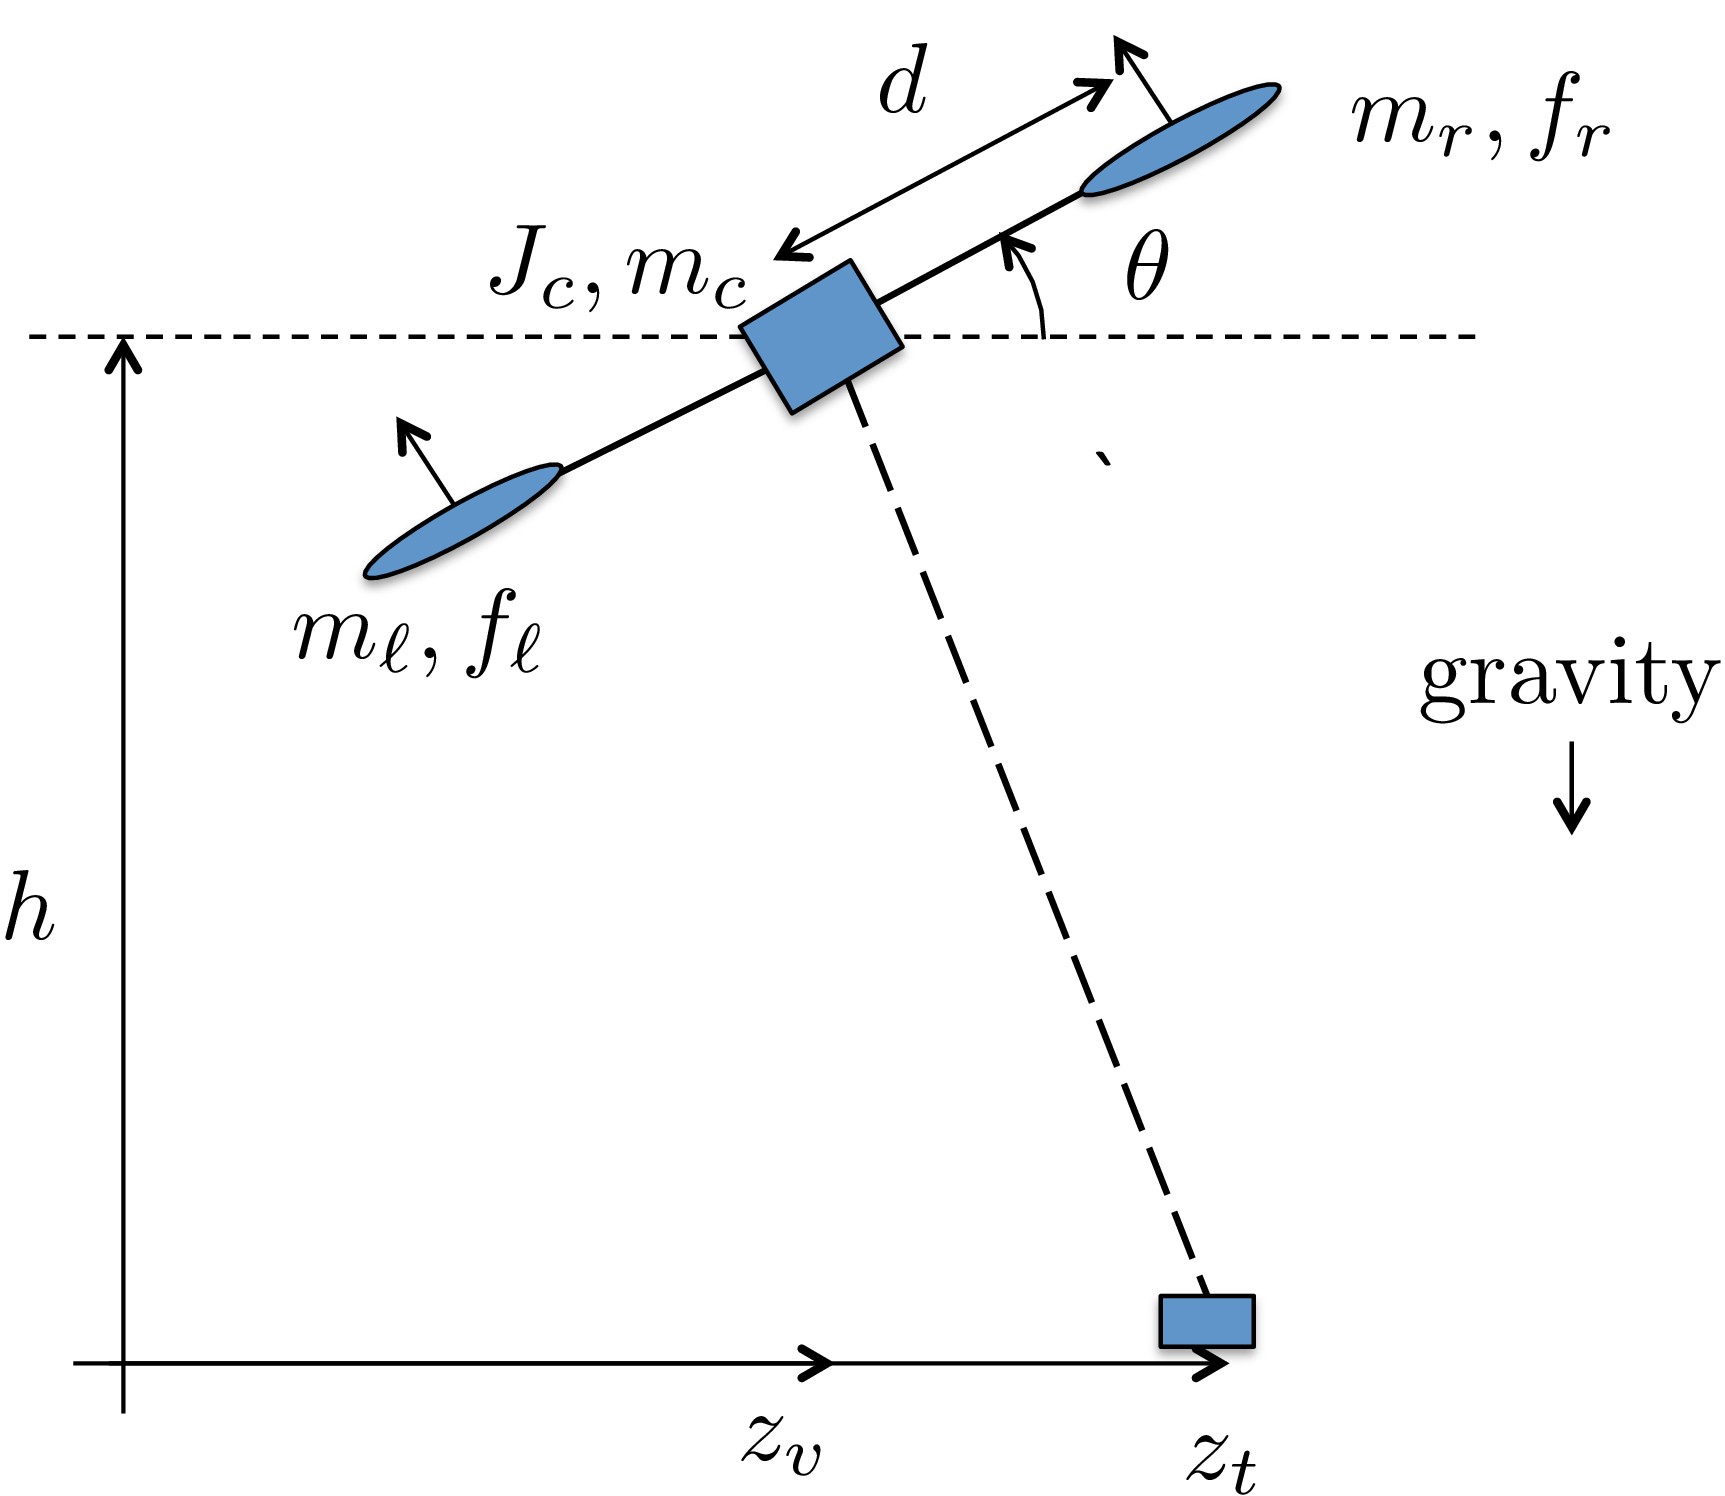
\includegraphics[width=0.59\textwidth]{6_design_studies/figures/hw_planar_VTOL_defn}\\
  \caption{Planar vertical take-off and landing (VTOL)}
  \label{fig:planar_VTOL_defn}
\end{wrapfigure}

In this design study we will explore the control design for a simplified planar version of a quadrotor following a ground target.  In particular, we will constrain the dynamics to be in two dimension plane comprising vertical and one dimension of horizontal, as shown in \fref{fig:planar_VTOL_defn}.  The planar vertical take-off and landing (VTOL) system is comprised of a center pod of mass $m_c$ and inertia $J_c$, a right motor/rotor that is modeled as a point mass $m_r$ that exerts a force $f_r$ at a distance $d$ from the center of mass, and a left motor/rotor that is modeled as a point mass $m_\ell$ that exerts a force $f_\ell$ at a distance $-d$ from the center of mass.  The position of the center of mass of the planar VTOL system is given by horizontal position $z_v$ and altitude $h$.  The airflow through the rotor creates a change in the direction of flow of air and causes what is called ``momentum drag.''  Momentum drag can be modeled as a viscous drag force that is proportional to the horizontal velocity $\dot{z}_v$.  In other words, the drag force is $F_{\text{drag}}=-\mu \dot{z}_v$.  The target on the ground will be modeled as an object with position $z_t$ and altitude $h=0$.  We will not explicitly model the dynamics of the target.  

Use the following physical parameters:
$m_c=1$~kg,
$J_c=0.0042$~kg m$^2$,
$m_r=0.25$~kg,
$m_\ell=0.25$~kg,
$d=0.3$~m,
$\mu = 0.1$~kg/s,
$g=9.81$~m/s$^2$.

